\documentclass[citenumber]{llncs}
%
\usepackage{makeidx}  % allows for indexgeneration
%
\usepackage{hyperref}				% enlaces en el pdf
\hypersetup{colorlinks=true,        % colores en vez de cajas en los enlaces
			linkcolor=blue,         % color of internal links (change box color with linkbordercolor)
    		citecolor=blue,         % color of links to bibliography
    		filecolor=blue,         % color of file links
    		urlcolor=blue}          % color of external links	    

\usepackage{algorithm}
\usepackage{setspace}				% Para el seudocódigo
\usepackage{amsmath}				% Para el seudocódigo
\usepackage[noend]{algpseudocode}	% Para el seudocódigo
\usepackage{multicol}				% Para el seudocódigo
\usepackage{graphicx}           	% para manejar imagenes
\usepackage[utf8]{inputenc}

\begin{document}
\mainmatter              % start of the contributions
%
\title{MLIT vs. Minreduct: a comparative study.}
			 
\author{Vlad\'{i}mir Rodr\'{i}guez--Diez\inst{1,2} \and Jos\'{e}~Fco. Mart\'{i}nez--Trinidad\inst{3}
		 \and J.~Ariel Carrasco--Ochoa\inst{3} \and Manuel~S.~Lazo--Cortés\inst{3} \and J. Arturo Olvera--López\inst{1}}
%
\authorrunning{Vlad\'{i}mir Rodr\'{i}guez et al.} % abbreviated author list (for running head)
%
\institute{Benemérita Universidad Autónoma de Puebla,\\
	Faculty of Computer Science,\\
	Language \& Knowledge Engineering Lab,\\
	Av. del Infante S/N, Ciudad Universitaria, Puebla, Pue. México\\
\and Universidad de Camag\"{u}ey,\\
	Circunvalaci\'{o}n Nte. km 5$\frac{1}{2}$, Camag\"{u}ey, Cuba\\
	\email{vladimir.rodriguez@reduc.edu.cu}
\and Instituto Nacional de Astrof\'{i}sica, \'{O}ptica y Electr\'{o}nica,\\
	 Luis Enrique Erro \# 1, Tonantzintla, Puebla, M\'{e}xico,\\
	 Coordinaci\'{o}n de Ciencias Computacionales,\\}


\maketitle              % typeset the title of the contribution

\begin{abstract}
	Rough set reducts are irreducible subsets of attributes preserving discernibility information of an decision system. Computing all reducts has exponential complexity regarding the number of attributes in the decision system. Given the high computational cost of this task, computing only the reducts of minimum length (the shortest reducts) becomes relevant for a wide range of applications. Two recent algorithms have been reported, almost simultaneously, for computing this irreducible subsets of attributes with minimum length: MLIT and Minreduct. MLIT was designed in the top of the Testor Theory while Minreduct comes from the Rough Set Theory. Both algorithms are intended to solve an equivalent algorithmic task. Thus, in this paper we present a comparative study of these algorithm in terms of asymptotic complexity and runtime performance. 
	
\keywords{Typical Testor, Reduct, minimum--length, shortest}
\end{abstract}
%
\section{Introduction}
%
	% Que son los TT, de donde vienen y cual es el problema de calcularlos
	
	Testors were originally created by Cheguis and Yablonskii \cite{Cheguis55} as a tool for analysis of problems connected with control and diagnosis of faults in electronic circuits.  Within Testor Theory, typical testors are irreducible subsets of attributes preserving the object discernibility ability of the original set of attributes. Thus, typical testors have been used for feature selection as shown in \cite{Dmitriev1966,Ruiz08}. Typical testors are needed for solving some real--world applications. For instance, in~\cite{Torres2014} the informational weight is used to identify risk factors on transfusion, related to acute lung injury; and to establish an assessment for each attribute. 
	
	Unfortunately, computing all typical testors from a dataset has exponential complexity regarding its number of attributes. Thus, the development of fast algorithms for typical testor computation have been an active research topic for more than three decades. One of the first algorithms for finding all typical testors, was proposed in \cite{Ruiz85} and modified in \cite{sanchez02}. This algorithm, called BT, codifies a subset of attributes as a binary word, and evaluates candidate subsets in the natural ascending order induced by the binary numbers.  In \cite{Shulcloper95b} the REC algorithm was presented. REC works directly over the dataset, handling a huge amount of superfluous information. Then, the CER algorithm~\cite{Ayaquica97}, overcomes this drawback and uses a different traversing order. Later, a new algorithm called LEX~\cite{Santiesteban03} was introduced. The key point of LEX was its new traversing order of candidates that resembles the lexicographical order in which character strings are compared. This traversing order was also followed by the subsequent reported algorithms: CT\_EXT~\cite{Sanchez07} and BR~\cite{Lias09}. The most recent algorithms reported for typical testor computation are the newest versions of these two algorithms: fast--CT\_EXT~\cite{Sanchez10} and fast--BR~\cite{Lias13}.
	
	% Relación con los trabajos de reductos
	
	Recently, reducts from the Rough Set Theory (RST) have been related to typical testors~\cite{Chikalov2013}. RST was proposed by Z. Pawlak in 1981 \cite{Pawlak81} as a mathematical theory to deal with imperfect knowledge, in particular with vague concepts. In~\cite{Lazo15}, it was proven that algorithms for reduct computation can be applied to typical testor computation, since these two concepts are equivalent for consistent datasets. In~\cite{Rodriguez2018}, the GCreduct algorithm for reduct computation was presented and it was evaluated against fast--CT\_EXT and fast--BR. In this work, it was concluded that GCreduct outperforms fast--CT\_EXT in all cases.
	
	% En este trabajose presenta un estudio...
	
	It is a well known fact that there is not one unique algorithm for computing typical testors having the best performance for every given problem. Most algorithms for computing typical testors operate over the basic matrix. The basic matrix is a reduced binary matrix representing the discernibility information of the dataset. Former studies~\cite{Lias13,Rodriguez15}, have performed experiments by categorizing the  basic matrices according to their density of 1's; i.e. the number of ones divided by the total number of cells of the matrix. In~\cite{Gonzalez15} it was concluded that  the performance of the algorithms for computing typical testors is related to the number of rows, the density of 1's and the number of typical testors of the basic matrix. In~\cite{Rodriguez2017} it was detailed a procedure for evaluating these algorithms over a synthetic sample of basic matrices with the same dimension and different density of 1's. This procedure was also followed in~\cite{Rodriguez2018}. As a next step, in this work, we present an experimental study on the effects of the basic matrix dimensions on the performance of the algorithms for typical testor computation. For our experiments we have selected fast--BR and GCreduct, since these algorithms are the most recent and fastest algorithms reported for typical testor (reduct) computation. The selected algorithms are first executed over a sample of synthetic basic matrices, and the conclusions drawn from this experiment are corroborated over real--world datasets taken from the UCI machine learning repository~\cite{Bache13}. 	
	
	% Estructura del documento
	
	The rest of this paper is structured in the following way. In Section~\ref{tb}, some basic concepts from Testor Theory are introduced and the pruning properties for typical testor computation are presented. In Section~\ref{Algs}, we describe both algorithms: GCreduct and fast--BR. Then, in Section~\ref{evaluation}, we present our experimental study and we discuss the results. Finally, our conclusions appear in Section~\ref{conclusions}.
	
	

					
%
\section{Theoretical background} \label{tb}
%

In this section, we introduce the main concepts of Testor Theory, as well as the definitions and propositions supporting the pruning strategies used in GCreduct and fast--BR. 

%
\subsection{Basic Concepts} \label{basic_concetps}
%

Let $DS$ be a dataset with $k$ objects described by $n$ attributes and grouped into $r$ classes. Every attribute in the set of attributes $R=\lbrace x_1,...,x_n \rbrace$, has a predefined Boolean comparison criterion. Let $DM$ be the binary comparison matrix obtained from comparing every pair of objects in $DS$ belonging to different classes. Every comparison of a pair of objects adds a row to $DM$ with 0=equal,1=different in the corresponding attribute position (column). $DM$ has $m$ rows and $n$ columns. Comparisons generating a row with only 0's, hereinafter referred to as empty row, imply that two objects from different classes are equal according to their attribute values. 

\begin{definition}\label{def:testor}
	Let $T \subseteq R$ be a subset of attributes from $DS$. T is a testor of DS (or DM) if in the sub-matrix of DM formed by the columns corresponding to attributes in T, there is not any empty row.
\end{definition} 	

Usually the number of rows in $DM$ ($m$) is large. In~\cite{Lazo01} a reduction of $DM$ without loss of relevant information was proposed, and in~\cite{Piza17} it was proved that this reduced matrix, called \textit{basic matrix} ($BM$), and $DM$; have the same set of testors. Then, we can substitute $DM$ by $BM$ in the definition~\ref{def:testor} without any loss of generality. 	

\begin{definition}\label{def:TT}
	A subset of attributes $T \subseteq R$ is a typical testor in BM iff T is a testor and $\forall x_i \in T, T \setminus x_i$ is not a testor. 
\end{definition}

%	
\subsection{Pruning properties for typical testor computation}
%

	The concept of contribution presented in Definition~\ref{def:contrib} is a key aspect for both algorithms: GCreduct and fast--BR. 	
	
	\begin{definition}\label{def:contrib}
		Given $T \subseteq R$ and $x_i \in R$ such that $x_i \notin T$. $x_i$ contributes to T iff the sub-matrix of BM formed with only those attributes in T has more empty rows than that matrix formed with attributes in $T \cup \lbrace x_i \rbrace$.
	\end{definition}	
	
	First introduced for the CT\_EXT algorithm, Proposition~\ref{prop:contrib} was stated and proved in~\cite{Sanchez10}.
	
	\begin{proposition}\label{prop:contrib} 
		Given $T \subseteq R$ and  $x_i \in R$ such that $x_i \notin T$. If $x_i$ does not contribute to T, then $T\cup\{x_i\}$ cannot be a subset of any typical testor.
	\end{proposition}
	
%	\begin{proposition}\label{prop:superset} 
%		Given $T \subseteq R$ and $Z \subseteq R$ such that $Z \cap T = \emptyset$. If T is a testor, then $T \cup Z$ is a testor too, but it is not a typical testor.
%	\end{proposition}

	The following propositions are stated and proved in~\cite{Lias13}.
	
	\begin{definition}\label{def:exclusion}
		Given $T \subseteq R$. The compatibility mask of $T$, denoted as $cm_T$, is the binary word in which the $j^{\mathit{th}}$ bit is 1 if the $j^{\mathit{th}}$ row of $BM$ has a 1 in only one of the columns corresponding to attributes in $T$, and otherwise it is 0.
	\end{definition}
	
	\begin{proposition}\label{prop:exclude} 
		Given $T \subseteq R$ and $x_i \in R$ such that $x_i \notin T$.	We denote as $c_{x_k}$ to the binary word in which the $j^{\mathit{th}}$ bit is 1 if the $j^{\mathit{th}}$ row of $BM$ has a 1 in the column corresponding to $x_k$. If $\exists x_k \in T$ such that $cm_{T \cup \lbrace x_i\rbrace} \wedge c_{x_k}=(0,...,0)$, then, $T \cup \lbrace x_i\rbrace$ cannot be a subset of any typical testor, and we will say that $x_i$ is exclusionary with $T$.
	\end{proposition}
	
	\begin{proposition}\label{prop:TT} 
		Given $T \subseteq R$ and $x_i \in R$ such that $x_i \notin T$. The subset $T \cup \lbrace x_i\rbrace$ is a typical testor iff it is a testor and $x_i$ is not exclusionary with $T$.
	\end{proposition}

	We will refer to Proposition~\ref{prop:exclude} as exclusion evaluation. Proposition~\ref{prop:TT} expresses how to apply the exclusion evaluation for determining whether or not a subset $T$ of attributes is a typical testor.
	
	The propositions presented in this section constitute the basis for understanding the differences between fast--BR and GCreduct. 
%
\section{MLIT and Minreduct algorithms} \label{Algs}
%
	In this section, we present a comparison of the candidate evaluation process of fast--BR and GCreduct. We aim to provide enough elements to understand the different performance of these two algorithms for a given dataset. It is important to highlight that both algorithms operate over the basic matrix. Thus, when referring to characteristics of the basic matrix, we are indeed referring also to characteristics of the dataset from which the basic matrix was computed.
	
	% Explicar el pseudocódigo de ambos en terminos de complejidad
	In GCreduct, a new candidate is generated by including a new attribute to the previous candidate. First, this new attribute is tested for contribution by using Definition~\ref{def:contrib}. This process has a time complexity $\Theta(m)$, where $m$ is the number of rows in the basic matrix. By Proposition~\ref{prop:contrib}, if the new attribute does not contribute to the candidate, this attribute is rejected. Otherwise, the candidate is evaluated for the testor condition by using Definition~\ref{def:testor}. This operation has also a time complexity $\Theta(m)$ as it was stated in~\cite{Rodriguez2018}. Then, for those candidates satisfying the testor condition, the exclusion evaluation is performed to determine whether  or not they are typical testors. This final verification is accomplished by means of Proposition~\ref{prop:TT}, and its time complexity is $\Theta(mn)$; where $n$ is the number of columns in the basic matrix.
	
	In fast--BR, a new candidate is also generated by including a new attribute to the previous candidate. In the same way, the first evaluation step for the candidate is the test for contribution of the new attribute, which has a time complexity $\Theta(m)$. However, for contributing candidates, the next step is the exclusion evaluation. This process is accomplished by means of Proposition~\ref{prop:exclude} and it has a time complexity $\Theta(mn)$. If the new attribute is exclusionary with the previous candidate, the attribute is rejected. Otherwise, the testor condition is verified by using Definition~\ref{def:testor}. This final process has a time complexity $\Theta(m)$. Those candidates evaluated as testors, in this candidate evaluation process, are also typical testors because of the order followed in this algorithm.
	
	% Hablar de las condiciones q son favorables a uno y otro desde la teoría
	
	In both algorithms, the candidate evaluation has a time complexity $\Theta(mn)$. Also, the total number of evaluated candidates has an exponential relation to the number of attributes in the dataset, for both algorithms. Thus, for both algorithms, the time complexity for typical testor computation is exponential. However, there are significant differences in the runtime of fast--BR and GCreduct for a given dataset. 
	
	The exclusion evaluation is the step with the highest time complexity in the candidate evaluation process for both algorithms. In GCreduct, this step is only executed for those candidates satisfying the testor condition, which are usually a small fraction of the total contributing candidates. In fast-BR, the exclusion evaluation is performed for every contributing candidate, which makes its candidate evaluation process more computationally expensive than GCreduct's. However, fast-BR takes advantage of this costly evaluation by discarding all the supersets of an exclusionary candidate by applying Proposition~\ref{prop:exclude}. This advantage is more effective for basic matrices with a higher density of 1's, as it was shown in~\cite{Rodriguez2018}.
%
\section{Comparative study} \label{evaluation}
%
\subsection{Complexity analysis of MinReduct}\label{complexity}
	
	 According to the main pruning property of the algorithm, candidates with length higher than the shortest reduct found so far are not evaluated. If the algorithm knows the length of the shortest reducts ($k$), the upper bound of the search space ($ss$) is the number of combinations that can be generated with length lower than or equal to $k$ with the number of attributes $n$. The asymptotic limit for this number of combinations is: 
	
	\begin{equation}
	ss= O\left( \sum_{i=1}^{k} \binom{n}{i} +f(n)\right)\label{eq:ss1}
	\end{equation}
	
	In Equation~\ref{eq:ss1}, $f(n)$ represents the number of combinations with length higher than $k$ that are evaluated before the first of the shortest reducts is found. There are many algorithms for computing $k$ in a time proportional to $n$ (this is what propose Lin, T. and Yin, P in our reference 16). Through the development of MinReduct our experiments showed that no statistically significant runtime reduction can be achieved when the algorithm knows beforehand the value of $k$. Thus, we did not include an approximate algorithm for determining the value of $k$ as an initial stage of MinReduct. Therefore, we simplify Equation~\ref{eq:ss1} as follows:
	
	\begin{equation}
	ss= O\left( \sum_{i=1}^{k} \binom{n}{i}\right)\label{eq:ss2}
	\end{equation}
	
	Because of Proposition 6, there are some combinations that have been counted in Equation~\ref{eq:ss2} which are not evaluated. If we denote by $n_0$ the number of zeros in the first row of the arranged basic matrix, those combinations can be excluded as follows:	
	
	\begin{equation}
	ss= O\left(\sum_{i=1}^{k} \binom{n}{i} - \sum_{i=1}^{\mathrm{min}(n_0,k)} \binom{n_0}{i}\right)\label{eq:ss3}
	\end{equation}
			
	Figure~\ref{fig:candidates} shows the \textbf{real} number of evaluated candidates and the \textbf{asymptotic upper bound} computed by Equation~\ref{eq:ss3} for the 500 synthetic matrices used in our experiments. Figure~\ref{fig:candidates} supports the validity of the expression obtained for $ss$.
	
	\begin{figure}[hbt] 
		\begin{center}
			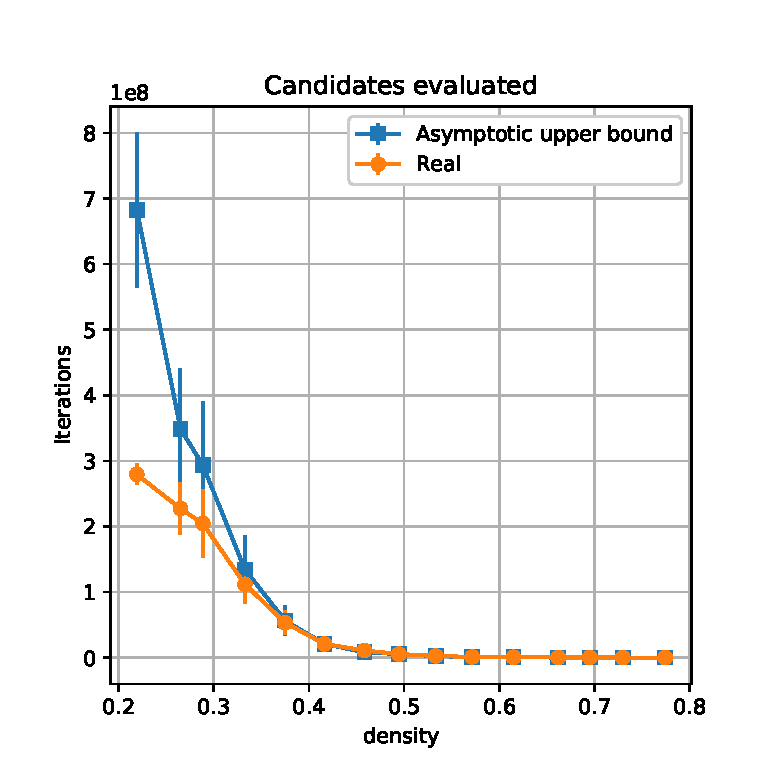
\includegraphics[height=4in]{Candidates_vs_SearchSpace.eps}
		\end{center}
		\caption{Evaluated candidates and search space as a function of the density.}\label{fig:candidates}
	\end{figure}  
	
	Candidate evaluation in MinReduct has a worst case time complexity of $\Theta(nm)$, for those combinations that require exclusion evaluation. For candidate combinations that do not include the last attribute of the arranged basic matrix ($c_{max}$) the time complexity of the evaluation is $\Theta(m)$ (lines 5--15 and 27--29). Notice that the length of the current candidate $|B+ [c]|$ can be cumulatively computed such that the time complexity of line 27 is $\Theta(1)$. For those combinations including $c_{max}$, the evaluation (lines 17--25) has a time complexity of $\Theta(nm)$ in the worst case. The number of combinations with length lower than or equal to $k$ that include $c_{max}$ ($ss_{c_{max}}$) has an asymptotic upper bound defined by the following expression:
	
	\begin{equation*}
	ss_{c_{max}}= O\left(\frac{1}{n-1}\sum_{i=1}^{k} \binom{n}{i} - \frac{1}{n_0-1}\sum_{i=1}^{\mathrm{min}(n_0,k)} \binom{n_0}{i}\right)\label{eq:c_max1}
	\end{equation*}
	\begin{equation}
	ss_{c_{max}}= O\left(\frac{1}{n}\sum_{i=1}^{k} \binom{n}{i} - \frac{1}{n_0}\sum_{i=1}^{\mathrm{min}(n_0,k)} \binom{n_0}{i}\right)\label{eq:c_max2}
	\end{equation}
	
	Thus, we can compute the upper bound of the asymptotic time complexity ($T$) for MinReduct by the following expression:
	
	\begin{equation}
	T = O\left(m*ss + mn*ss_{c_{max}}\label{eq:T1}\right)
	\end{equation}
	
	\begin{equation*}
	T = O\left(m\left[\sum_{i=1}^{k} \binom{n}{i} - \sum_{i=1}^{\mathrm{min}(n_0,k)} \binom{n_0}{i}\right]+mn\left[\frac{1}{n}\sum_{i=1}^{k} \binom{n}{i} - \frac{1}{n_0}\sum_{i=1}^{\mathrm{min}(n_0,k)} \binom{n_0}{i}\right]\right)
	\end{equation*}	
	
	\begin{equation}
	T = O\left(m\left[2\sum_{i=1}^{k} \binom{n}{i} - \left(1 + \frac{n}{n_0}\right)\sum_{i=1}^{\mathrm{min}(n_0,k)} \binom{n_0}{i}\right]\right)\label{eq:T2}
	\end{equation}	
	
	Figure~\ref{fig:n0} shows the behavior of  $k$ and $n_0$ as a function of the density for the 500 synthetic matrices used in our experiments. This behavior, together with Equation~\ref{eq:T2} illustrates the reason for the relatively low cost of computing reducts in matrices with a high density of ones.
		
	\begin{figure}[hbt]
		\begin{center}
			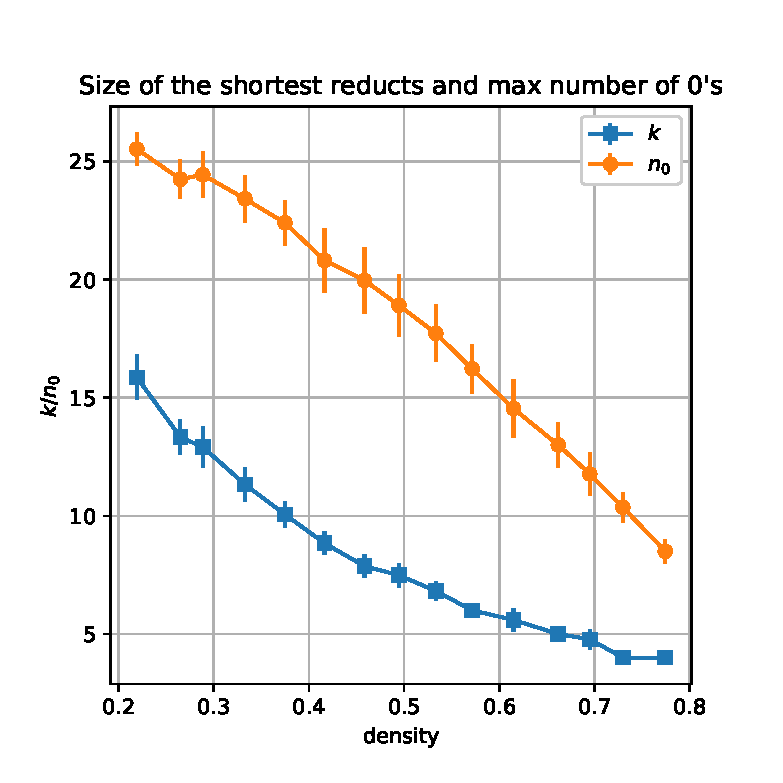
\includegraphics[height=4in]{Length_and_N0_vs_denisty.eps} 
		\end{center}
		\caption{Behavior of $k$ and $n_0$ as a function of the density of the basic matrix.}\label{fig:n0}
	\end{figure}  
	
	Space complexity of MinReduct consist of two main components: the space required for storing the set of all the shortest reducts, and the space required for the candidate evaluation. The number of elements in set of all the shortest reducts is exponentially related to $n$. The space required for candidate evaluation in MinReduct is $\Theta(mn)$ because of the evaluations are performed in--place.
	
	A more compact analysis of the algorithm's complexity was included in the section~3 of the paper in order to attend the editor comment.
%
\subsection{Experimental comparison}\label{Comparison}
%	
	We thankfully acknowledge the authors of MLIT for sharing the source code of their Java implementations of the MLIT algorithm. 	
	
	\begin{figure}[hbt]
		\begin{center}
			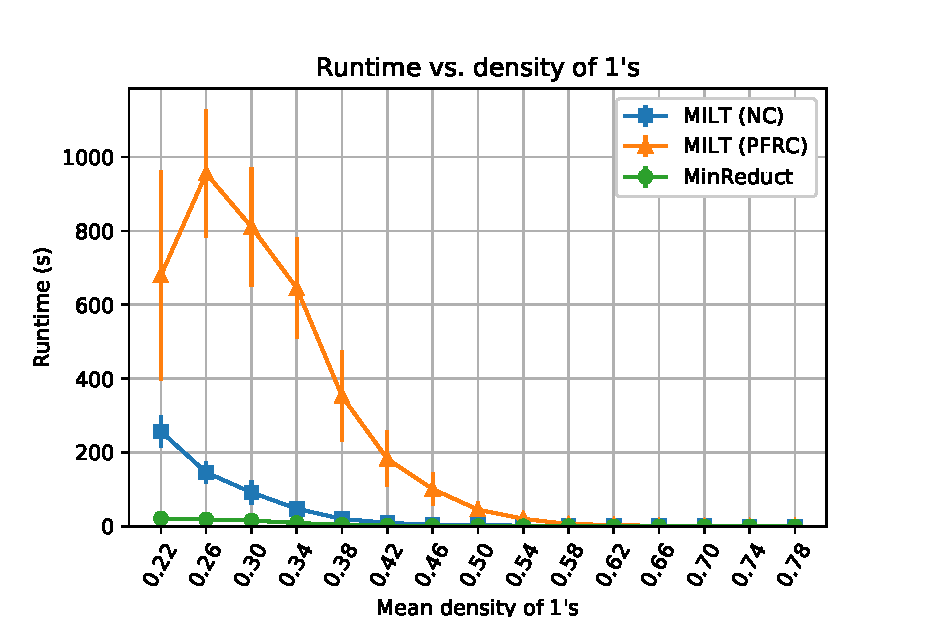
\includegraphics[height=3in]{MinReduct_vs_milt.eps} 
		\end{center}
		\caption{Average runtime vs. density of 1’s for MinReduct and MLIT.}\label{fig:sinthyetic}
	\end{figure}  		
	
	Figure~\ref{fig:sinthyetic} shows the average runtime for MLIT (NC and PFRC) and MinReduct as a function of the density of 1’s in the 500 synthetic basic matrices used in the paper. This experiment was carried out under the same conditions of the experiments exposed in the paper. As it can be seen in Figure~\ref{fig:sinthyetic}, MLIT was not faster than MinReduct in any case. 			
	
	\begin{table}[htb]
		\small
		\caption{Runtime over synthetic basic matrices.}
		\centering
		\begin{tabular}{lcccccccc}\label{tab:comparison}
			Dimension & density & Len & Nsol & MinReduct & MLIT(NC) & MLIT(PFRC)\\
			\hline
			250x600  & 0.84 & 2 &   170  &      0.269     & \textbf{0.104} &  0.127 \\
			1500x150 & 0.75 & 4 & 228778 & \textbf{2.286} &     21.998     & 37.855 \\
		\end{tabular}             
	\end{table}  
	
	Table~\ref{tab:comparison} shows the runtime of MLIT (NC and PFRC) and MinReduct for two matrices with dimensions (rows x attributes) 250x600 and 1500x150, with densities 0.84 and 0.75 respectively. These are the last two matrices requested by the editor. For the matrix with 1200 rows and 110 attributes with density 0.33, the solution could not be obtained so far by any of the algorithms. Thus, from this basic matrix, the last columns were removed in order to obtain sub--matrices with a lower number of columns. Figure~\ref{fig:1200x110}  shows the runtime of MLIT (NC and PFRC) and MinReduct for the matrices with 1200 rows and density 0.33 with a number of columns between 30 and 54. 
	
	\begin{figure}[hbt]
		\begin{center}
			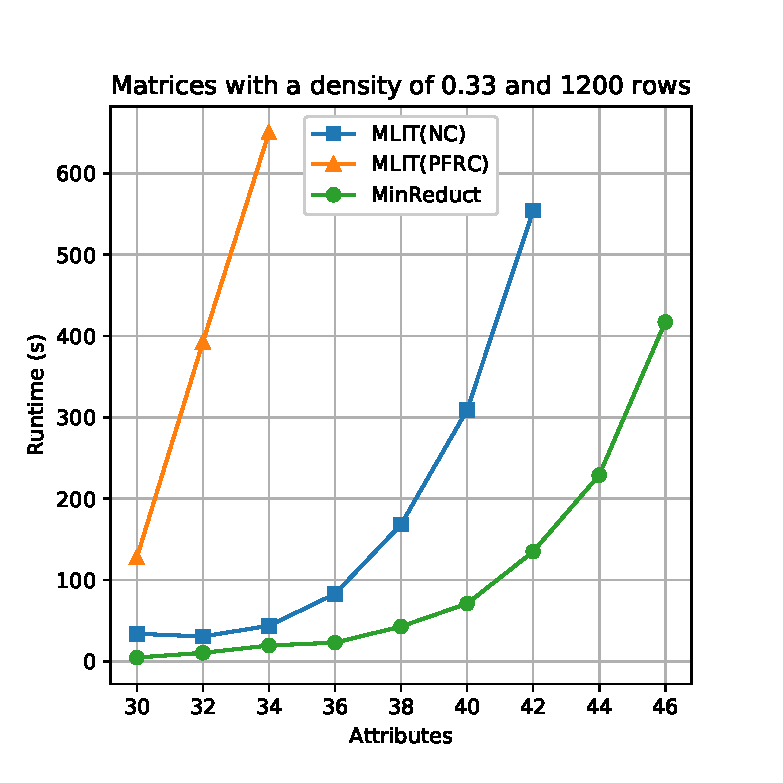
\includegraphics[height=4in]{low_density_Minreduct_vs_MLIT.eps} 
		\end{center}
		\caption{Runtime for matrices with 1200 rows and density 0.33.}\label{fig:1200x110}
	\end{figure}  
	
	As a result of these experiments carried out over 515 synthetic matrices,  MLIT (NC) was faster than MinReduct in 10 matrices. These 10 matrices have a density higher or equal to 0.6 and its runtime is below one second. The PFRC version of MLIT was faster than MinReduct in one matrix and it was never the fastest algorithm. 
	
	It is important to highlight that the PFRC version of MLIT performs systematically slower than the NC version in our experiments as well as in their authors' experiments.  MLIT (NC) evaluates all the combinations in the search space defined by Equation~\ref{eq:ss3} (Altough their authors refer in their paper a number of combinations equivalent to Equation~\ref{eq:ss2}) without using any pruning property. The PFRC version, on the other hand, incorporates pruning rules over the feature power set to make fewer evaluations; which seems to be no so efficient in practice. A breadth-first search for finding all the shortest reducts, as in MLIT, guarantees that no combination with length higher than $k$ is evaluated. But, as it was disused before, there is no significant advantage in having such restriction of the search space. However, applying pruning rules in a breadth-first search is less efficient in term of both: time and space, than the traditional depth-first search used in most algorithms for reduct computation. From the asymptotic complexity point of view, MinReduct (Equation~\ref{eq:T2}) is at least $k/2$ faster than MLIT (NC) \cite{Piza20}. 
	
	This relation between the runtime of MinReduct and MLIT (NC) can be experimentally corroborated taking the values of $k$ from Figure~\ref{fig:n0} and the runtimes shown in Figure~\ref{fig:sinthyetic}.
%
\section{Conclusions} \label{conclusions}
%	
	%TODO dar umbrales
	In this paper, we have explored the relation between the dimensions of the basic matrix associated to a dataset and the performance of fast-BR and GCreduct. These are the most recent and fastest algorithms reported for typical testor (reduct) computation. Previous studies found that the density of 1's in the basic matrix can be used to determine a priori the fastest algorithm for a given dataset. In addition, we have found in this work, that basic matrices with a high number of rows are favorable for GCreduct, in the same manner that a high number of attributes makes a dataset better suited for fast--BR. Thus, the boundary density dividing the datasets for which each algorithm has the best performance should be computed taking into account the basic matrix dimension.
	
	Finally, we corroborated our results obtained from synthetic datasets over a set of real--world datasets taken from the UCI machine learning repository. These results allowed explaining the behavior of the two algorithms better than just using the density of 1's in the basic matrix.
	
	For future work, we propose performing a deeper and wider experimentation in order to define a rule to determine which algorithm would be the best for a specific dataset	
 
%
\section{Acknowledgments} \label{Acknowledgements}
%
	This work was partly supported by National Council of Science and Technology of Mexico under the scholarship grant 399547.

% ---- Bibliography ----
%
\bibliography{mybib}{}
\bibliographystyle{splncs03}

\end{document}
